\documentclass[1p]{elsarticle_modified}
%\bibliographystyle{elsarticle-num}

%\usepackage[colorlinks]{hyperref}
%\usepackage{abbrmath_seonhwa} %\Abb, \Ascr, \Acal ,\Abf, \Afrak
\usepackage{amsfonts}
\usepackage{amssymb}
\usepackage{amsmath}
\usepackage{amsthm}
\usepackage{scalefnt}
\usepackage{amsbsy}
\usepackage{kotex}
\usepackage{caption}
\usepackage{subfig}
\usepackage{color}
\usepackage{graphicx}
\usepackage{xcolor} %% white, black, red, green, blue, cyan, magenta, yellow
\usepackage{float}
\usepackage{setspace}
\usepackage{hyperref}

\usepackage{tikz}
\usetikzlibrary{arrows}

\usepackage{multirow}
\usepackage{array} % fixed length table
\usepackage{hhline}

%%%%%%%%%%%%%%%%%%%%%
\makeatletter
\renewcommand*\env@matrix[1][\arraystretch]{%
	\edef\arraystretch{#1}%
	\hskip -\arraycolsep
	\let\@ifnextchar\new@ifnextchar
	\array{*\c@MaxMatrixCols c}}
\makeatother %https://tex.stackexchange.com/questions/14071/how-can-i-increase-the-line-spacing-in-a-matrix
%%%%%%%%%%%%%%%

\usepackage[normalem]{ulem}

\newcommand{\msout}[1]{\ifmmode\text{\sout{\ensuremath{#1}}}\else\sout{#1}\fi}
%SOURCE: \msout is \stkout macro in https://tex.stackexchange.com/questions/20609/strikeout-in-math-mode

\newcommand{\cancel}[1]{
	\ifmmode
	{\color{red}\msout{#1}}
	\else
	{\color{red}\sout{#1}}
	\fi
}

\newcommand{\add}[1]{
	{\color{blue}\uwave{#1}}
}

\newcommand{\replace}[2]{
	\ifmmode
	{\color{red}\msout{#1}}{\color{blue}\uwave{#2}}
	\else
	{\color{red}\sout{#1}}{\color{blue}\uwave{#2}}
	\fi
}

\newcommand{\Sol}{\mathcal{S}} %segment
\newcommand{\D}{D} %diagram
\newcommand{\A}{\mathcal{A}} %arc


%%%%%%%%%%%%%%%%%%%%%%%%%%%%%5 test

\def\sl{\operatorname{\textup{SL}}(2,\Cbb)}
\def\psl{\operatorname{\textup{PSL}}(2,\Cbb)}
\def\quan{\mkern 1mu \triangleright \mkern 1mu}

\theoremstyle{definition}
\newtheorem{thm}{Theorem}[section]
\newtheorem{prop}[thm]{Proposition}
\newtheorem{lem}[thm]{Lemma}
\newtheorem{ques}[thm]{Question}
\newtheorem{cor}[thm]{Corollary}
\newtheorem{defn}[thm]{Definition}
\newtheorem{exam}[thm]{Example}
\newtheorem{rmk}[thm]{Remark}
\newtheorem{alg}[thm]{Algorithm}

\newcommand{\I}{\sqrt{-1}}
\begin{document}

%\begin{frontmatter}
%
%\title{Boundary parabolic representations of knots up to 8 crossings}
%
%%% Group authors per affiliation:
%\author{Yunhi Cho} 
%\address{Department of Mathematics, University of Seoul, Seoul, Korea}
%\ead{yhcho@uos.ac.kr}
%
%
%\author{Seonhwa Kim} %\fnref{s_kim}}
%\address{Center for Geometry and Physics, Institute for Basic Science, Pohang, 37673, Korea}
%\ead{ryeona17@ibs.re.kr}
%
%\author{Hyuk Kim}
%\address{Department of Mathematical Sciences, Seoul National University, Seoul 08826, Korea}
%\ead{hyukkim@snu.ac.kr}
%
%\author{Seokbeom Yoon}
%\address{Department of Mathematical Sciences, Seoul National University, Seoul, 08826,  Korea}
%\ead{sbyoon15@snu.ac.kr}
%
%\begin{abstract}
%We find all boundary parabolic representation of knots up to 8 crossings.
%
%\end{abstract}
%\begin{keyword}
%    \MSC[2010] 57M25 
%\end{keyword}
%
%\end{frontmatter}

%\linenumbers
%\tableofcontents
%
\newcommand\colored[1]{\textcolor{white}{\rule[-0.35ex]{0.8em}{1.4ex}}\kern-0.8em\color{red} #1}%
%\newcommand\colored[1]{\textcolor{white}{ #1}\kern-2.17ex	\textcolor{white}{ #1}\kern-1.81ex	\textcolor{white}{ #1}\kern-2.15ex\color{red}#1	}

{\Large $\underline{12n_{0606}~(K12n_{0606})}$}

\setlength{\tabcolsep}{10pt}
\renewcommand{\arraystretch}{1.6}
\vspace{1cm}\begin{tabular}{m{100pt}>{\centering\arraybackslash}m{274pt}}
\multirow{5}{120pt}{
	\centering
	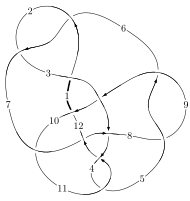
\includegraphics[width=112pt]{../../../GIT/diagram.site/Diagrams/png/2695_12n_0606.png}\\
\ \ \ A knot diagram\footnotemark}&
\allowdisplaybreaks
\textbf{Linearized knot diagam} \\
\cline{2-2}
 &
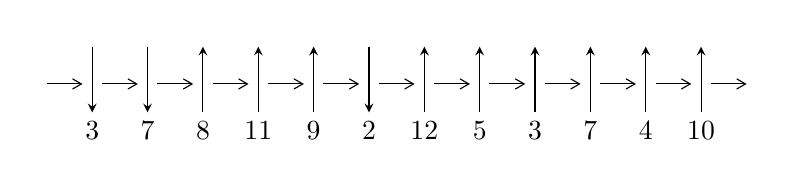
\begin{tikzpicture}[x=20pt, y=17pt]
	% nodes
	\node (C0) at (0, 0) {};
	\node (C1) at (1, 0) {};
	\node (C1U) at (1, +1) {};
	\node (C1D) at (1, -1) {3};

	\node (C2) at (2, 0) {};
	\node (C2U) at (2, +1) {};
	\node (C2D) at (2, -1) {7};

	\node (C3) at (3, 0) {};
	\node (C3U) at (3, +1) {};
	\node (C3D) at (3, -1) {8};

	\node (C4) at (4, 0) {};
	\node (C4U) at (4, +1) {};
	\node (C4D) at (4, -1) {11};

	\node (C5) at (5, 0) {};
	\node (C5U) at (5, +1) {};
	\node (C5D) at (5, -1) {9};

	\node (C6) at (6, 0) {};
	\node (C6U) at (6, +1) {};
	\node (C6D) at (6, -1) {2};

	\node (C7) at (7, 0) {};
	\node (C7U) at (7, +1) {};
	\node (C7D) at (7, -1) {12};

	\node (C8) at (8, 0) {};
	\node (C8U) at (8, +1) {};
	\node (C8D) at (8, -1) {5};

	\node (C9) at (9, 0) {};
	\node (C9U) at (9, +1) {};
	\node (C9D) at (9, -1) {3};

	\node (C10) at (10, 0) {};
	\node (C10U) at (10, +1) {};
	\node (C10D) at (10, -1) {7};

	\node (C11) at (11, 0) {};
	\node (C11U) at (11, +1) {};
	\node (C11D) at (11, -1) {4};

	\node (C12) at (12, 0) {};
	\node (C12U) at (12, +1) {};
	\node (C12D) at (12, -1) {10};
	\node (C13) at (13, 0) {};

	% arrows
	\draw[->,>={angle 60}]
	(C0) edge (C1) (C1) edge (C2) (C2) edge (C3) (C3) edge (C4) (C4) edge (C5) (C5) edge (C6) (C6) edge (C7) (C7) edge (C8) (C8) edge (C9) (C9) edge (C10) (C10) edge (C11) (C11) edge (C12) (C12) edge (C13) ;	\draw[->,>=stealth]
	(C1U) edge (C1D) (C2U) edge (C2D) (C3D) edge (C3U) (C4D) edge (C4U) (C5D) edge (C5U) (C6U) edge (C6D) (C7D) edge (C7U) (C8D) edge (C8U) (C9D) edge (C9U) (C10D) edge (C10U) (C11D) edge (C11U) (C12D) edge (C12U) ;
	\end{tikzpicture} \\
\hhline{~~} \\& 
\textbf{Solving Sequence} \\ \cline{2-2} 
 &
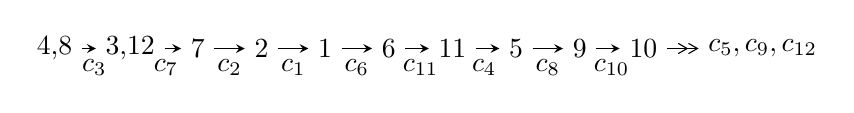
\begin{tikzpicture}[x=23pt, y=7pt]
	% node
	\node (A0) at (-1/8, 0) {4,8};
	\node (A1) at (17/16, 0) {3,12};
	\node (A2) at (17/8, 0) {7};
	\node (A3) at (25/8, 0) {2};
	\node (A4) at (33/8, 0) {1};
	\node (A5) at (41/8, 0) {6};
	\node (A6) at (49/8, 0) {11};
	\node (A7) at (57/8, 0) {5};
	\node (A8) at (65/8, 0) {9};
	\node (A9) at (73/8, 0) {10};
	\node (C1) at (1/2, -1) {$c_{3}$};
	\node (C2) at (13/8, -1) {$c_{7}$};
	\node (C3) at (21/8, -1) {$c_{2}$};
	\node (C4) at (29/8, -1) {$c_{1}$};
	\node (C5) at (37/8, -1) {$c_{6}$};
	\node (C6) at (45/8, -1) {$c_{11}$};
	\node (C7) at (53/8, -1) {$c_{4}$};
	\node (C8) at (61/8, -1) {$c_{8}$};
	\node (C9) at (69/8, -1) {$c_{10}$};
	\node (A10) at (11, 0) {$c_{5},c_{9},c_{12}$};

	% edge
	\draw[->,>=stealth]	
	(A0) edge (A1) (A1) edge (A2) (A2) edge (A3) (A3) edge (A4) (A4) edge (A5) (A5) edge (A6) (A6) edge (A7) (A7) edge (A8) (A8) edge (A9) ;
	\draw[->>,>={angle 60}]	
	(A9) edge (A10);
\end{tikzpicture} \\ 

\end{tabular} \\

\footnotetext{
The image of knot diagram is generated by the software ``\textbf{Draw programme}" developed by Andrew Bartholomew(\url{http://www.layer8.co.uk/maths/draw/index.htm\#Running-draw}), where we modified some parts for our purpose(\url{https://github.com/CATsTAILs/LinksPainter}).
}\phantom \\ \newline 
\centering \textbf{Ideals for irreducible components\footnotemark of $X_{\text{par}}$} 
 
\begin{align*}
I^u_{1}&=\langle 
-1.60434\times10^{191} u^{60}+3.06370\times10^{190} u^{59}+\cdots+9.90808\times10^{192} b-1.81924\times10^{193},\\
\phantom{I^u_{1}}&\phantom{= \langle  }1.45667\times10^{192} u^{60}-2.33309\times10^{192} u^{59}+\cdots+1.98162\times10^{193} a+2.73135\times10^{192},\;u^{61}- u^{60}+\cdots+58 u+25\rangle \\
I^u_{2}&=\langle 
6183716894369 u^{21}+1374457475661 u^{20}+\cdots+20376431428799 b-1818725790068,\\
\phantom{I^u_{2}}&\phantom{= \langle  }23344139331015 u^{21}+15115284063805 u^{20}+\cdots+40752862857598 a+81671293633640,\\
\phantom{I^u_{2}}&\phantom{= \langle  }u^{22}+u^{20}+\cdots+7 u^2+1\rangle \\
\\
\end{align*}
\raggedright * 2 irreducible components of $\dim_{\mathbb{C}}=0$, with total 83 representations.\\
\footnotetext{All coefficients of polynomials are rational numbers. But the coefficients are sometimes approximated in decimal forms when there is not enough margin.}
\newpage
\renewcommand{\arraystretch}{1}
\centering \section*{I. $I^u_{1}= \langle -1.60\times10^{191} u^{60}+3.06\times10^{190} u^{59}+\cdots+9.91\times10^{192} b-1.82\times10^{193},\;1.46\times10^{192} u^{60}-2.33\times10^{192} u^{59}+\cdots+1.98\times10^{193} a+2.73\times10^{192},\;u^{61}- u^{60}+\cdots+58 u+25 \rangle$}
\flushleft \textbf{(i) Arc colorings}\\
\begin{tabular}{m{7pt} m{180pt} m{7pt} m{180pt} }
\flushright $a_{4}=$&$\begin{pmatrix}1\\0\end{pmatrix}$ \\
\flushright $a_{8}=$&$\begin{pmatrix}0\\u\end{pmatrix}$ \\
\flushright $a_{3}=$&$\begin{pmatrix}1\\u^2\end{pmatrix}$ \\
\flushright $a_{12}=$&$\begin{pmatrix}-0.0735091 u^{60}+0.117737 u^{59}+\cdots-2.04132 u-0.137835\\0.0161923 u^{60}-0.00309212 u^{59}+\cdots+4.89491 u+1.83612\end{pmatrix}$ \\
\flushright $a_{7}=$&$\begin{pmatrix}0.139781 u^{60}-0.129132 u^{59}+\cdots+15.7191 u+4.33924\\-0.00116829 u^{60}+0.0144033 u^{59}+\cdots+1.86244 u+0.197937\end{pmatrix}$ \\
\flushright $a_{2}=$&$\begin{pmatrix}0.0704268 u^{60}-0.0732087 u^{59}+\cdots+2.42540 u+0.360156\\0.0813783 u^{60}-0.0764120 u^{59}+\cdots+12.8465 u+2.33043\end{pmatrix}$ \\
\flushright $a_{1}=$&$\begin{pmatrix}0.178777 u^{60}-0.179760 u^{59}+\cdots+16.8712 u+2.62104\\0.0511130 u^{60}-0.0380784 u^{59}+\cdots+10.0334 u+2.28547\end{pmatrix}$ \\
\flushright $a_{6}=$&$\begin{pmatrix}0.103262 u^{60}-0.0386507 u^{59}+\cdots+17.0502 u+9.16938\\-0.172371 u^{60}+0.154684 u^{59}+\cdots-24.1023 u-5.29676\end{pmatrix}$ \\
\flushright $a_{11}=$&$\begin{pmatrix}-0.0897013 u^{60}+0.120829 u^{59}+\cdots-6.93623 u-1.97395\\0.0161923 u^{60}-0.00309212 u^{59}+\cdots+4.89491 u+1.83612\end{pmatrix}$ \\
\flushright $a_{5}=$&$\begin{pmatrix}0.0660658 u^{60}-0.0890977 u^{59}+\cdots+6.16157 u-0.139445\\-0.0739833 u^{60}+0.0958469 u^{59}+\cdots-5.82769 u+1.54267\end{pmatrix}$ \\
\flushright $a_{9}=$&$\begin{pmatrix}-0.0689463 u^{60}+0.140243 u^{59}+\cdots-1.52496 u+4.30676\\0.0119356 u^{60}-0.0639002 u^{59}+\cdots-6.32232 u-5.61607\end{pmatrix}$ \\
\flushright $a_{10}=$&$\begin{pmatrix}-0.0431325 u^{60}+0.0739412 u^{59}+\cdots-5.43574 u+0.473106\\0.0113729 u^{60}-0.0535091 u^{59}+\cdots-4.61936 u-4.60387\end{pmatrix}$\\&\end{tabular}
\flushleft \textbf{(ii) Obstruction class $= -1$}\\~\\
\flushleft \textbf{(iii) Cusp Shapes $= 0.625154 u^{60}-0.710423 u^{59}+\cdots+55.0401 u+12.7589$}\\~\\
\newpage\renewcommand{\arraystretch}{1}
\flushleft \textbf{(iv) u-Polynomials at the component}\newline \\
\begin{tabular}{m{50pt}|m{274pt}}
Crossings & \hspace{64pt}u-Polynomials at each crossing \\
\hline $$\begin{aligned}c_{1}\end{aligned}$$&$\begin{aligned}
&u^{61}+80 u^{60}+\cdots+86779 u+2401
\end{aligned}$\\
\hline $$\begin{aligned}c_{2},c_{6}\end{aligned}$$&$\begin{aligned}
&u^{61}-2 u^{60}+\cdots+441 u-49
\end{aligned}$\\
\hline $$\begin{aligned}c_{3}\end{aligned}$$&$\begin{aligned}
&u^{61}+u^{60}+\cdots+58 u-25
\end{aligned}$\\
\hline $$\begin{aligned}c_{4},c_{11}\end{aligned}$$&$\begin{aligned}
&u^{61}-2 u^{60}+\cdots-33 u-19
\end{aligned}$\\
\hline $$\begin{aligned}c_{5},c_{8}\end{aligned}$$&$\begin{aligned}
&u^{61}-2 u^{60}+\cdots+261 u-29
\end{aligned}$\\
\hline $$\begin{aligned}c_{7}\end{aligned}$$&$\begin{aligned}
&u^{61}+2 u^{60}+\cdots-276 u-333
\end{aligned}$\\
\hline $$\begin{aligned}c_{9}\end{aligned}$$&$\begin{aligned}
&u^{61}-2 u^{60}+\cdots+96105 u-40873
\end{aligned}$\\
\hline $$\begin{aligned}c_{10}\end{aligned}$$&$\begin{aligned}
&u^{61}+2 u^{60}+\cdots-3730060 u-1063025
\end{aligned}$\\
\hline $$\begin{aligned}c_{12}\end{aligned}$$&$\begin{aligned}
&u^{61}+u^{60}+\cdots+24262 u-3637
\end{aligned}$\\
\hline
\end{tabular}\\~\\
\newpage\renewcommand{\arraystretch}{1}
\flushleft \textbf{(v) Riley Polynomials at the component}\newline \\
\begin{tabular}{m{50pt}|m{274pt}}
Crossings & \hspace{64pt}Riley Polynomials at each crossing \\
\hline $$\begin{aligned}c_{1}\end{aligned}$$&$\begin{aligned}
&y^{61}-188 y^{60}+\cdots-978957329 y-5764801
\end{aligned}$\\
\hline $$\begin{aligned}c_{2},c_{6}\end{aligned}$$&$\begin{aligned}
&y^{61}-80 y^{60}+\cdots+86779 y-2401
\end{aligned}$\\
\hline $$\begin{aligned}c_{3}\end{aligned}$$&$\begin{aligned}
&y^{61}+9 y^{60}+\cdots-4186 y-625
\end{aligned}$\\
\hline $$\begin{aligned}c_{4},c_{11}\end{aligned}$$&$\begin{aligned}
&y^{61}+42 y^{60}+\cdots+367 y-361
\end{aligned}$\\
\hline $$\begin{aligned}c_{5},c_{8}\end{aligned}$$&$\begin{aligned}
&y^{61}-24 y^{60}+\cdots+17197 y-841
\end{aligned}$\\
\hline $$\begin{aligned}c_{7}\end{aligned}$$&$\begin{aligned}
&y^{61}+24 y^{60}+\cdots-3453624 y-110889
\end{aligned}$\\
\hline $$\begin{aligned}c_{9}\end{aligned}$$&$\begin{aligned}
&y^{61}+106 y^{60}+\cdots-28850843549 y-1670602129
\end{aligned}$\\
\hline $$\begin{aligned}c_{10}\end{aligned}$$&$\begin{aligned}
&y^{61}+50 y^{60}+\cdots+4847404798650 y-1130022150625
\end{aligned}$\\
\hline $$\begin{aligned}c_{12}\end{aligned}$$&$\begin{aligned}
&y^{61}+83 y^{60}+\cdots-463357606 y-13227769
\end{aligned}$\\
\hline
\end{tabular}\\~\\
\newpage\flushleft \textbf{(vi) Complex Volumes and Cusp Shapes}
$$\begin{array}{c|c|c}  
\text{Solutions to }I^u_{1}& \I (\text{vol} + \sqrt{-1}CS) & \text{Cusp shape}\\
 \hline 
\begin{aligned}
u &= -0.910345 + 0.431030 I \\
a &= \phantom{-}0.083295 - 0.454008 I \\
b &= \phantom{-}0.591145 + 0.176936 I\end{aligned}
 & \phantom{-}2.26261 - 0.47311 I & \phantom{-}6.00000 + 0.82328 I \\ \hline\begin{aligned}
u &= -0.910345 - 0.431030 I \\
a &= \phantom{-}0.083295 + 0.454008 I \\
b &= \phantom{-}0.591145 - 0.176936 I\end{aligned}
 & \phantom{-}2.26261 + 0.47311 I & \phantom{-}6.00000 - 0.82328 I \\ \hline\begin{aligned}
u &= -0.905896 + 0.155656 I \\
a &= -0.855256 + 0.495486 I \\
b &= -0.471322 + 0.022876 I\end{aligned}
 & \phantom{-}1.384080 - 0.049647 I & \phantom{-}8.60374 + 0.34198 I \\ \hline\begin{aligned}
u &= -0.905896 - 0.155656 I \\
a &= -0.855256 - 0.495486 I \\
b &= -0.471322 - 0.022876 I\end{aligned}
 & \phantom{-}1.384080 + 0.049647 I & \phantom{-}8.60374 - 0.34198 I \\ \hline\begin{aligned}
u &= \phantom{-}0.873224 + 0.669571 I \\
a &= \phantom{-}0.981899 + 0.270500 I \\
b &= \phantom{-}0.849049 - 0.003724 I\end{aligned}
 & \phantom{-}0.68598 + 5.02449 I & \phantom{-}6.00000 - 6.97083 I \\ \hline\begin{aligned}
u &= \phantom{-}0.873224 - 0.669571 I \\
a &= \phantom{-}0.981899 - 0.270500 I \\
b &= \phantom{-}0.849049 + 0.003724 I\end{aligned}
 & \phantom{-}0.68598 - 5.02449 I & \phantom{-}6.00000 + 6.97083 I \\ \hline\begin{aligned}
u &= \phantom{-}0.796281 + 0.378338 I \\
a &= -1.116940 - 0.754299 I \\
b &= -0.339467 - 1.155790 I\end{aligned}
 & -2.21988 + 2.71821 I & \phantom{-}2.79760 - 2.35403 I \\ \hline\begin{aligned}
u &= \phantom{-}0.796281 - 0.378338 I \\
a &= -1.116940 + 0.754299 I \\
b &= -0.339467 + 1.155790 I\end{aligned}
 & -2.21988 - 2.71821 I & \phantom{-}2.79760 + 2.35403 I \\ \hline\begin{aligned}
u &= -0.783728 + 0.810034 I \\
a &= -1.086800 + 0.185128 I \\
b &= -1.269080 - 0.034183 I\end{aligned}
 & -8.29039 - 8.79817 I & \phantom{-0.000000 -}0. + 5.94350 I \\ \hline\begin{aligned}
u &= -0.783728 - 0.810034 I \\
a &= -1.086800 - 0.185128 I \\
b &= -1.269080 + 0.034183 I\end{aligned}
 & -8.29039 + 8.79817 I & \phantom{-0.000000 } 0. - 5.94350 I\\
 \hline 
 \end{array}$$\newpage$$\begin{array}{c|c|c}  
\text{Solutions to }I^u_{1}& \I (\text{vol} + \sqrt{-1}CS) & \text{Cusp shape}\\
 \hline 
\begin{aligned}
u &= \phantom{-}1.100430 + 0.405618 I \\
a &= \phantom{-}0.564804 - 0.867691 I \\
b &= \phantom{-}0.668724 - 0.343543 I\end{aligned}
 & -7.18810 + 2.78232 I & \phantom{-0.000000 } 0 \\ \hline\begin{aligned}
u &= \phantom{-}1.100430 - 0.405618 I \\
a &= \phantom{-}0.564804 + 0.867691 I \\
b &= \phantom{-}0.668724 + 0.343543 I\end{aligned}
 & -7.18810 - 2.78232 I & \phantom{-0.000000 } 0 \\ \hline\begin{aligned}
u &= \phantom{-}0.902535 + 0.787150 I \\
a &= \phantom{-}1.38806 + 0.58993 I \\
b &= \phantom{-}0.077875 + 1.023620 I\end{aligned}
 & -2.49063 + 3.37367 I & \phantom{-0.000000 } 0 \\ \hline\begin{aligned}
u &= \phantom{-}0.902535 - 0.787150 I \\
a &= \phantom{-}1.38806 - 0.58993 I \\
b &= \phantom{-}0.077875 - 1.023620 I\end{aligned}
 & -2.49063 - 3.37367 I & \phantom{-0.000000 } 0 \\ \hline\begin{aligned}
u &= -0.143701 + 1.197970 I \\
a &= -0.758684 - 0.050261 I \\
b &= -0.81574 - 1.26237 I\end{aligned}
 & -12.04860 + 3.96320 I & \phantom{-0.000000 } 0 \\ \hline\begin{aligned}
u &= -0.143701 - 1.197970 I \\
a &= -0.758684 + 0.050261 I \\
b &= -0.81574 + 1.26237 I\end{aligned}
 & -12.04860 - 3.96320 I & \phantom{-0.000000 } 0 \\ \hline\begin{aligned}
u &= -0.737649 + 0.288030 I \\
a &= -1.22841 + 1.53957 I \\
b &= \phantom{-}0.141796 + 0.826845 I\end{aligned}
 & \phantom{-}1.16799 + 0.97942 I & \phantom{-}11.64968 - 5.59628 I \\ \hline\begin{aligned}
u &= -0.737649 - 0.288030 I \\
a &= -1.22841 - 1.53957 I \\
b &= \phantom{-}0.141796 - 0.826845 I\end{aligned}
 & \phantom{-}1.16799 - 0.97942 I & \phantom{-}11.64968 + 5.59628 I \\ \hline\begin{aligned}
u &= \phantom{-}0.409288 + 1.166070 I \\
a &= -0.968903 + 0.296598 I \\
b &= -0.873837 - 0.531957 I\end{aligned}
 & -10.15910 + 2.60373 I & \phantom{-0.000000 } 0 \\ \hline\begin{aligned}
u &= \phantom{-}0.409288 - 1.166070 I \\
a &= -0.968903 - 0.296598 I \\
b &= -0.873837 + 0.531957 I\end{aligned}
 & -10.15910 - 2.60373 I & \phantom{-0.000000 } 0\\
 \hline 
 \end{array}$$\newpage$$\begin{array}{c|c|c}  
\text{Solutions to }I^u_{1}& \I (\text{vol} + \sqrt{-1}CS) & \text{Cusp shape}\\
 \hline 
\begin{aligned}
u &= -0.178219 + 1.234730 I \\
a &= \phantom{-}0.704583 + 0.086186 I \\
b &= \phantom{-}0.489122 - 1.159650 I\end{aligned}
 & -4.94617 - 1.68496 I & \phantom{-0.000000 } 0 \\ \hline\begin{aligned}
u &= -0.178219 - 1.234730 I \\
a &= \phantom{-}0.704583 - 0.086186 I \\
b &= \phantom{-}0.489122 + 1.159650 I\end{aligned}
 & -4.94617 + 1.68496 I & \phantom{-0.000000 } 0 \\ \hline\begin{aligned}
u &= \phantom{-}0.548172 + 0.498732 I \\
a &= -0.827761 - 0.239428 I \\
b &= -1.175910 + 0.324455 I\end{aligned}
 & \phantom{-}3.56437 + 0.65529 I & \phantom{-}6.54598 - 9.43946 I \\ \hline\begin{aligned}
u &= \phantom{-}0.548172 - 0.498732 I \\
a &= -0.827761 + 0.239428 I \\
b &= -1.175910 - 0.324455 I\end{aligned}
 & \phantom{-}3.56437 - 0.65529 I & \phantom{-}6.54598 + 9.43946 I \\ \hline\begin{aligned}
u &= -0.783796 + 0.998521 I \\
a &= -1.48491 + 0.19075 I \\
b &= -0.301845 + 1.321410 I\end{aligned}
 & -15.6806 - 6.1080 I & \phantom{-0.000000 } 0 \\ \hline\begin{aligned}
u &= -0.783796 - 0.998521 I \\
a &= -1.48491 - 0.19075 I \\
b &= -0.301845 - 1.321410 I\end{aligned}
 & -15.6806 + 6.1080 I & \phantom{-0.000000 } 0 \\ \hline\begin{aligned}
u &= -0.514875 + 0.492130 I \\
a &= \phantom{-}1.59948 + 2.11483 I \\
b &= \phantom{-}0.398091 - 1.052590 I\end{aligned}
 & -9.26345 - 6.82861 I & \phantom{-}3.46166 + 7.84368 I \\ \hline\begin{aligned}
u &= -0.514875 - 0.492130 I \\
a &= \phantom{-}1.59948 - 2.11483 I \\
b &= \phantom{-}0.398091 + 1.052590 I\end{aligned}
 & -9.26345 + 6.82861 I & \phantom{-}3.46166 - 7.84368 I \\ \hline\begin{aligned}
u &= \phantom{-}0.264074 + 0.645372 I \\
a &= \phantom{-}1.328340 + 0.443782 I \\
b &= -0.016093 + 1.164140 I\end{aligned}
 & -3.08605 - 2.29569 I & \phantom{-}1.42347 + 3.66981 I \\ \hline\begin{aligned}
u &= \phantom{-}0.264074 - 0.645372 I \\
a &= \phantom{-}1.328340 - 0.443782 I \\
b &= -0.016093 - 1.164140 I\end{aligned}
 & -3.08605 + 2.29569 I & \phantom{-}1.42347 - 3.66981 I\\
 \hline 
 \end{array}$$\newpage$$\begin{array}{c|c|c}  
\text{Solutions to }I^u_{1}& \I (\text{vol} + \sqrt{-1}CS) & \text{Cusp shape}\\
 \hline 
\begin{aligned}
u &= \phantom{-}0.773573 + 1.049630 I \\
a &= \phantom{-}1.183780 + 0.080595 I \\
b &= \phantom{-}0.573481 + 1.240910 I\end{aligned}
 & -4.00356 + 7.17574 I & \phantom{-0.000000 } 0 \\ \hline\begin{aligned}
u &= \phantom{-}0.773573 - 1.049630 I \\
a &= \phantom{-}1.183780 - 0.080595 I \\
b &= \phantom{-}0.573481 - 1.240910 I\end{aligned}
 & -4.00356 - 7.17574 I & \phantom{-0.000000 } 0 \\ \hline\begin{aligned}
u &= -0.338814 + 1.265940 I \\
a &= -0.521179 + 0.796599 I \\
b &= \phantom{-}0.139314 - 0.503690 I\end{aligned}
 & -9.74367 + 3.57994 I & \phantom{-0.000000 } 0 \\ \hline\begin{aligned}
u &= -0.338814 - 1.265940 I \\
a &= -0.521179 - 0.796599 I \\
b &= \phantom{-}0.139314 + 0.503690 I\end{aligned}
 & -9.74367 - 3.57994 I & \phantom{-0.000000 } 0 \\ \hline\begin{aligned}
u &= -0.308314 + 0.613085 I \\
a &= \phantom{-}1.345220 + 0.160561 I \\
b &= \phantom{-}0.935401 + 0.570302 I\end{aligned}
 & -1.34263 - 1.55470 I & \phantom{-}1.10269 + 5.91362 I \\ \hline\begin{aligned}
u &= -0.308314 - 0.613085 I \\
a &= \phantom{-}1.345220 - 0.160561 I \\
b &= \phantom{-}0.935401 - 0.570302 I\end{aligned}
 & -1.34263 + 1.55470 I & \phantom{-}1.10269 - 5.91362 I \\ \hline\begin{aligned}
u &= -0.122393 + 0.642085 I \\
a &= \phantom{-}1.260040 + 0.577361 I \\
b &= \phantom{-}0.488074 + 0.349651 I\end{aligned}
 & -1.49067 - 1.69118 I & \phantom{-}1.10870 + 3.00446 I \\ \hline\begin{aligned}
u &= -0.122393 - 0.642085 I \\
a &= \phantom{-}1.260040 - 0.577361 I \\
b &= \phantom{-}0.488074 - 0.349651 I\end{aligned}
 & -1.49067 + 1.69118 I & \phantom{-}1.10870 - 3.00446 I \\ \hline\begin{aligned}
u &= -0.846285 + 1.110770 I \\
a &= -0.848090 + 0.034436 I \\
b &= -0.62079 + 1.29122 I\end{aligned}
 & \phantom{-}0.31756 - 6.96705 I & \phantom{-0.000000 } 0 \\ \hline\begin{aligned}
u &= -0.846285 - 1.110770 I \\
a &= -0.848090 - 0.034436 I \\
b &= -0.62079 - 1.29122 I\end{aligned}
 & \phantom{-}0.31756 + 6.96705 I & \phantom{-0.000000 } 0\\
 \hline 
 \end{array}$$\newpage$$\begin{array}{c|c|c}  
\text{Solutions to }I^u_{1}& \I (\text{vol} + \sqrt{-1}CS) & \text{Cusp shape}\\
 \hline 
\begin{aligned}
u &= -0.203948 + 0.521772 I \\
a &= -2.18101 - 1.13787 I \\
b &= \phantom{-}0.195182 + 0.839910 I\end{aligned}
 & \phantom{-}1.01441 + 1.12155 I & \phantom{-}11.43554 + 3.06720 I \\ \hline\begin{aligned}
u &= -0.203948 - 0.521772 I \\
a &= -2.18101 + 1.13787 I \\
b &= \phantom{-}0.195182 - 0.839910 I\end{aligned}
 & \phantom{-}1.01441 - 1.12155 I & \phantom{-}11.43554 - 3.06720 I \\ \hline\begin{aligned}
u &= -0.075463 + 0.501572 I \\
a &= -1.70075 + 0.64346 I \\
b &= -0.47776 + 1.67863 I\end{aligned}
 & -13.75710 + 1.91932 I & -2.60893 - 4.18261 I \\ \hline\begin{aligned}
u &= -0.075463 - 0.501572 I \\
a &= -1.70075 - 0.64346 I \\
b &= -0.47776 - 1.67863 I\end{aligned}
 & -13.75710 - 1.91932 I & -2.60893 + 4.18261 I \\ \hline\begin{aligned}
u &= \phantom{-}1.20031 + 0.90858 I \\
a &= -0.708252 - 0.230947 I \\
b &= -0.317542 - 1.245240 I\end{aligned}
 & -2.34363 + 3.20308 I & \phantom{-0.000000 } 0 \\ \hline\begin{aligned}
u &= \phantom{-}1.20031 - 0.90858 I \\
a &= -0.708252 + 0.230947 I \\
b &= -0.317542 + 1.245240 I\end{aligned}
 & -2.34363 - 3.20308 I & \phantom{-0.000000 } 0 \\ \hline\begin{aligned}
u &= -0.441996\phantom{ +0.000000I} \\
a &= -1.57855\phantom{ +0.000000I} \\
b &= -0.366410\phantom{ +0.000000I}\end{aligned}
 & \phantom{-}0.849580\phantom{ +0.000000I} & \phantom{-}12.6400\phantom{ +0.000000I} \\ \hline\begin{aligned}
u &= \phantom{-}0.360834 + 0.209871 I \\
a &= -2.67749 + 1.83256 I \\
b &= -0.229649 - 0.967482 I\end{aligned}
 & -0.79546 + 2.56100 I & \phantom{-}5.10158 - 6.10959 I \\ \hline\begin{aligned}
u &= \phantom{-}0.360834 - 0.209871 I \\
a &= -2.67749 - 1.83256 I \\
b &= -0.229649 + 0.967482 I\end{aligned}
 & -0.79546 - 2.56100 I & \phantom{-}5.10158 + 6.10959 I \\ \hline\begin{aligned}
u &= -1.62571 + 0.49135 I \\
a &= -0.031980 + 0.495894 I \\
b &= \phantom{-}0.09176 + 1.50621 I\end{aligned}
 & -13.41560 - 0.23117 I & \phantom{-0.000000 } 0\\
 \hline 
 \end{array}$$\newpage$$\begin{array}{c|c|c}  
\text{Solutions to }I^u_{1}& \I (\text{vol} + \sqrt{-1}CS) & \text{Cusp shape}\\
 \hline 
\begin{aligned}
u &= -1.62571 - 0.49135 I \\
a &= -0.031980 - 0.495894 I \\
b &= \phantom{-}0.09176 - 1.50621 I\end{aligned}
 & -13.41560 + 0.23117 I & \phantom{-0.000000 } 0 \\ \hline\begin{aligned}
u &= \phantom{-}1.10477 + 1.32184 I \\
a &= -0.921810 - 0.135912 I \\
b &= -0.59623 - 1.40084 I\end{aligned}
 & -12.6177 + 15.2705 I & \phantom{-0.000000 } 0 \\ \hline\begin{aligned}
u &= \phantom{-}1.10477 - 1.32184 I \\
a &= -0.921810 + 0.135912 I \\
b &= -0.59623 + 1.40084 I\end{aligned}
 & -12.6177 - 15.2705 I & \phantom{-0.000000 } 0 \\ \hline\begin{aligned}
u &= -1.21132 + 1.26115 I \\
a &= \phantom{-}0.809022 - 0.138932 I \\
b &= \phantom{-}0.447860 - 1.318690 I\end{aligned}
 & -3.42883 - 9.78730 I & \phantom{-0.000000 } 0 \\ \hline\begin{aligned}
u &= -1.21132 - 1.26115 I \\
a &= \phantom{-}0.809022 + 0.138932 I \\
b &= \phantom{-}0.447860 + 1.318690 I\end{aligned}
 & -3.42883 + 9.78730 I & \phantom{-0.000000 } 0 \\ \hline\begin{aligned}
u &= \phantom{-}1.23693 + 1.30689 I \\
a &= \phantom{-}0.413103 + 0.160610 I \\
b &= \phantom{-}0.357957 + 1.350540 I\end{aligned}
 & -1.82315 + 4.26546 I & \phantom{-0.000000 } 0 \\ \hline\begin{aligned}
u &= \phantom{-}1.23693 - 1.30689 I \\
a &= \phantom{-}0.413103 - 0.160610 I \\
b &= \phantom{-}0.357957 - 1.350540 I\end{aligned}
 & -1.82315 - 4.26546 I & \phantom{-0.000000 } 0 \\ \hline\begin{aligned}
u &= -0.77616 + 1.81286 I \\
a &= \phantom{-}0.418912 - 0.019439 I \\
b &= \phantom{-}0.057249 - 1.068760 I\end{aligned}
 & -4.52908 - 0.45066 I & \phantom{-0.000000 } 0 \\ \hline\begin{aligned}
u &= -0.77616 - 1.81286 I \\
a &= \phantom{-}0.418912 + 0.019439 I \\
b &= \phantom{-}0.057249 + 1.068760 I\end{aligned}
 & -4.52908 + 0.45066 I & \phantom{-0.000000 } 0 \\ \hline\begin{aligned}
u &= \phantom{-}1.61718 + 1.51372 I \\
a &= -0.213047 - 0.314323 I \\
b &= \phantom{-}0.186383 - 1.117350 I\end{aligned}
 & -11.73450 - 5.28579 I & \phantom{-0.000000 } 0\\
 \hline 
 \end{array}$$\newpage$$\begin{array}{c|c|c}  
\text{Solutions to }I^u_{1}& \I (\text{vol} + \sqrt{-1}CS) & \text{Cusp shape}\\
 \hline 
\begin{aligned}
u &= \phantom{-}1.61718 - 1.51372 I \\
a &= -0.213047 + 0.314323 I \\
b &= \phantom{-}0.186383 + 1.117350 I\end{aligned}
 & -11.73450 + 5.28579 I & \phantom{-0.000000 } 0\\
 \hline 
 \end{array}$$\newpage\newpage\renewcommand{\arraystretch}{1}
\centering \section*{II. $I^u_{2}= \langle 6.18\times10^{12} u^{21}+1.37\times10^{12} u^{20}+\cdots+2.04\times10^{13} b-1.82\times10^{12},\;2.33\times10^{13} u^{21}+1.51\times10^{13} u^{20}+\cdots+4.08\times10^{13} a+8.17\times10^{13},\;u^{22}+u^{20}+\cdots+7 u^2+1 \rangle$}
\flushleft \textbf{(i) Arc colorings}\\
\begin{tabular}{m{7pt} m{180pt} m{7pt} m{180pt} }
\flushright $a_{4}=$&$\begin{pmatrix}1\\0\end{pmatrix}$ \\
\flushright $a_{8}=$&$\begin{pmatrix}0\\u\end{pmatrix}$ \\
\flushright $a_{3}=$&$\begin{pmatrix}1\\u^2\end{pmatrix}$ \\
\flushright $a_{12}=$&$\begin{pmatrix}-0.572822 u^{21}-0.370901 u^{20}+\cdots-6.42292 u-2.00406\\-0.303474 u^{21}-0.0674533 u^{20}+\cdots-2.11438 u+0.0892563\end{pmatrix}$ \\
\flushright $a_{7}=$&$\begin{pmatrix}-0.490404 u^{21}+0.544286 u^{20}+\cdots+1.63604 u+3.54751\\0.450223 u^{21}+0.166556 u^{20}+\cdots+1.84761 u+0.395045\end{pmatrix}$ \\
\flushright $a_{2}=$&$\begin{pmatrix}0.127478 u^{21}-0.0969833 u^{20}+\cdots-2.82648 u-1.83138\\-0.272013 u^{21}-0.162826 u^{20}+\cdots-3.02486 u-0.530692\end{pmatrix}$ \\
\flushright $a_{1}=$&$\begin{pmatrix}-0.160976 u^{21}-0.342532 u^{20}+\cdots-5.72386 u-2.45906\\-0.0738264 u^{21}-0.215757 u^{20}+\cdots-2.73641 u-0.285144\end{pmatrix}$ \\
\flushright $a_{6}=$&$\begin{pmatrix}-0.902443 u^{21}+0.369937 u^{20}+\cdots-3.12076 u+1.80659\\-0.508034 u^{21}+0.236676 u^{20}+\cdots-2.08651 u-0.447991\end{pmatrix}$ \\
\flushright $a_{11}=$&$\begin{pmatrix}-0.269348 u^{21}-0.303448 u^{20}+\cdots-4.30854 u-2.09332\\-0.303474 u^{21}-0.0674533 u^{20}+\cdots-2.11438 u+0.0892563\end{pmatrix}$ \\
\flushright $a_{5}=$&$\begin{pmatrix}0.224994 u^{21}+0.335014 u^{20}+\cdots-1.53934 u+1.95806\\-0.620039 u^{21}+0.115209 u^{20}+\cdots-2.49559 u-0.110441\end{pmatrix}$ \\
\flushright $a_{9}=$&$\begin{pmatrix}-0.843674 u^{21}+0.135737 u^{20}+\cdots-1.44434 u+0.954289\\0.0771103 u^{21}+0.230053 u^{20}+\cdots+0.290077 u+0.454193\end{pmatrix}$ \\
\flushright $a_{10}=$&$\begin{pmatrix}-0.798104 u^{21}+0.208278 u^{20}+\cdots-1.99794 u+1.54422\\-0.0334405 u^{21}+0.446821 u^{20}+\cdots+0.244507 u+0.381653\end{pmatrix}$\\&\end{tabular}
\flushleft \textbf{(ii) Obstruction class $= 1$}\\~\\
\flushleft \textbf{(iii) Cusp Shapes $= \frac{40525880426923}{40752862857598} u^{21}+\frac{9112819862999}{40752862857598} u^{20}+\cdots-\frac{281490623171531}{40752862857598} u+\frac{94744620113174}{20376431428799}$}\\~\\
\newpage\renewcommand{\arraystretch}{1}
\flushleft \textbf{(iv) u-Polynomials at the component}\newline \\
\begin{tabular}{m{50pt}|m{274pt}}
Crossings & \hspace{64pt}u-Polynomials at each crossing \\
\hline $$\begin{aligned}c_{1}\end{aligned}$$&$\begin{aligned}
&u^{22}-23 u^{21}+\cdots-11 u+1
\end{aligned}$\\
\hline $$\begin{aligned}c_{2}\end{aligned}$$&$\begin{aligned}
&u^{22}- u^{21}+\cdots+u+1
\end{aligned}$\\
\hline $$\begin{aligned}c_{3}\end{aligned}$$&$\begin{aligned}
&u^{22}+u^{20}+\cdots+7 u^2+1
\end{aligned}$\\
\hline $$\begin{aligned}c_{4}\end{aligned}$$&$\begin{aligned}
&u^{22}+u^{21}+\cdots+u+7
\end{aligned}$\\
\hline $$\begin{aligned}c_{5}\end{aligned}$$&$\begin{aligned}
&u^{22}- u^{21}+\cdots-3 u+5
\end{aligned}$\\
\hline $$\begin{aligned}c_{6}\end{aligned}$$&$\begin{aligned}
&u^{22}+u^{21}+\cdots- u+1
\end{aligned}$\\
\hline $$\begin{aligned}c_{7}\end{aligned}$$&$\begin{aligned}
&u^{22}+u^{21}+\cdots-4 u+1
\end{aligned}$\\
\hline $$\begin{aligned}c_{8}\end{aligned}$$&$\begin{aligned}
&u^{22}+u^{21}+\cdots+3 u+5
\end{aligned}$\\
\hline $$\begin{aligned}c_{9}\end{aligned}$$&$\begin{aligned}
&u^{22}- u^{21}+\cdots+u+1
\end{aligned}$\\
\hline $$\begin{aligned}c_{10}\end{aligned}$$&$\begin{aligned}
&u^{22}+u^{21}+\cdots-10 u+1
\end{aligned}$\\
\hline $$\begin{aligned}c_{11}\end{aligned}$$&$\begin{aligned}
&u^{22}- u^{21}+\cdots- u+7
\end{aligned}$\\
\hline $$\begin{aligned}c_{12}\end{aligned}$$&$\begin{aligned}
&u^{22}+6 u^{20}+\cdots-5 u^2+1
\end{aligned}$\\
\hline
\end{tabular}\\~\\
\newpage\renewcommand{\arraystretch}{1}
\flushleft \textbf{(v) Riley Polynomials at the component}\newline \\
\begin{tabular}{m{50pt}|m{274pt}}
Crossings & \hspace{64pt}Riley Polynomials at each crossing \\
\hline $$\begin{aligned}c_{1}\end{aligned}$$&$\begin{aligned}
&y^{22}-39 y^{21}+\cdots-3 y+1
\end{aligned}$\\
\hline $$\begin{aligned}c_{2},c_{6}\end{aligned}$$&$\begin{aligned}
&y^{22}-23 y^{21}+\cdots-11 y+1
\end{aligned}$\\
\hline $$\begin{aligned}c_{3}\end{aligned}$$&$\begin{aligned}
&y^{22}+2 y^{21}+\cdots+14 y+1
\end{aligned}$\\
\hline $$\begin{aligned}c_{4},c_{11}\end{aligned}$$&$\begin{aligned}
&y^{22}+15 y^{21}+\cdots+377 y+49
\end{aligned}$\\
\hline $$\begin{aligned}c_{5},c_{8}\end{aligned}$$&$\begin{aligned}
&y^{22}-19 y^{21}+\cdots-289 y+25
\end{aligned}$\\
\hline $$\begin{aligned}c_{7}\end{aligned}$$&$\begin{aligned}
&y^{22}+9 y^{21}+\cdots-4 y+1
\end{aligned}$\\
\hline $$\begin{aligned}c_{9}\end{aligned}$$&$\begin{aligned}
&y^{22}+15 y^{21}+\cdots+21 y+1
\end{aligned}$\\
\hline $$\begin{aligned}c_{10}\end{aligned}$$&$\begin{aligned}
&y^{22}+15 y^{21}+\cdots+38 y+1
\end{aligned}$\\
\hline $$\begin{aligned}c_{12}\end{aligned}$$&$\begin{aligned}
&y^{22}+12 y^{21}+\cdots-10 y+1
\end{aligned}$\\
\hline
\end{tabular}\\~\\
\newpage\flushleft \textbf{(vi) Complex Volumes and Cusp Shapes}
$$\begin{array}{c|c|c}  
\text{Solutions to }I^u_{2}& \I (\text{vol} + \sqrt{-1}CS) & \text{Cusp shape}\\
 \hline 
\begin{aligned}
u &= \phantom{-}0.749223 + 0.536697 I \\
a &= -1.93401 - 0.91661 I \\
b &= -0.274538 - 0.968002 I\end{aligned}
 & -1.82723 + 4.27576 I & \phantom{-}7.30430 - 9.72989 I \\ \hline\begin{aligned}
u &= \phantom{-}0.749223 - 0.536697 I \\
a &= -1.93401 + 0.91661 I \\
b &= -0.274538 + 0.968002 I\end{aligned}
 & -1.82723 - 4.27576 I & \phantom{-}7.30430 + 9.72989 I \\ \hline\begin{aligned}
u &= -1.044190 + 0.356102 I \\
a &= -0.001977 - 0.673618 I \\
b &= \phantom{-}0.26050 - 1.56100 I\end{aligned}
 & -12.82310 + 1.58068 I & \phantom{-}4.83519 - 2.88611 I \\ \hline\begin{aligned}
u &= -1.044190 - 0.356102 I \\
a &= -0.001977 + 0.673618 I \\
b &= \phantom{-}0.26050 + 1.56100 I\end{aligned}
 & -12.82310 - 1.58068 I & \phantom{-}4.83519 + 2.88611 I \\ \hline\begin{aligned}
u &= \phantom{-}0.724340 + 0.845777 I \\
a &= -0.821898 - 0.205533 I \\
b &= -0.988487 + 0.528451 I\end{aligned}
 & \phantom{-}1.66671 + 2.20771 I & \phantom{-}4.34569 - 3.65314 I \\ \hline\begin{aligned}
u &= \phantom{-}0.724340 - 0.845777 I \\
a &= -0.821898 + 0.205533 I \\
b &= -0.988487 - 0.528451 I\end{aligned}
 & \phantom{-}1.66671 - 2.20771 I & \phantom{-}4.34569 + 3.65314 I \\ \hline\begin{aligned}
u &= -1.046380 + 0.423272 I \\
a &= -0.356014 + 1.178150 I \\
b &= \phantom{-}0.173677 + 0.903500 I\end{aligned}
 & \phantom{-}0.651107 + 0.405045 I & \phantom{-}1.85611 + 1.13547 I \\ \hline\begin{aligned}
u &= -1.046380 - 0.423272 I \\
a &= -0.356014 - 1.178150 I \\
b &= \phantom{-}0.173677 - 0.903500 I\end{aligned}
 & \phantom{-}0.651107 - 0.405045 I & \phantom{-}1.85611 - 1.13547 I \\ \hline\begin{aligned}
u &= \phantom{-}0.558979 + 1.026050 I \\
a &= -0.045467 + 0.826842 I \\
b &= \phantom{-}0.431345 - 0.856577 I\end{aligned}
 & -9.94231 - 5.09085 I & \phantom{-}2.90449 + 4.36039 I \\ \hline\begin{aligned}
u &= \phantom{-}0.558979 - 1.026050 I \\
a &= -0.045467 - 0.826842 I \\
b &= \phantom{-}0.431345 + 0.856577 I\end{aligned}
 & -9.94231 + 5.09085 I & \phantom{-}2.90449 - 4.36039 I\\
 \hline 
 \end{array}$$\newpage$$\begin{array}{c|c|c}  
\text{Solutions to }I^u_{2}& \I (\text{vol} + \sqrt{-1}CS) & \text{Cusp shape}\\
 \hline 
\begin{aligned}
u &= -0.791899 + 0.115857 I \\
a &= \phantom{-}0.458376 - 0.091009 I \\
b &= \phantom{-}0.915727 + 0.059496 I\end{aligned}
 & \phantom{-}3.54705 - 0.01004 I & \phantom{-}10.61413 - 1.28755 I \\ \hline\begin{aligned}
u &= -0.791899 - 0.115857 I \\
a &= \phantom{-}0.458376 + 0.091009 I \\
b &= \phantom{-}0.915727 - 0.059496 I\end{aligned}
 & \phantom{-}3.54705 + 0.01004 I & \phantom{-}10.61413 + 1.28755 I \\ \hline\begin{aligned}
u &= \phantom{-}0.231354 + 0.517578 I \\
a &= -0.34516 - 2.70664 I \\
b &= \phantom{-}0.205725 + 0.843817 I\end{aligned}
 & \phantom{-}0.70306 + 1.50488 I & \phantom{-}1.38672 - 8.70491 I \\ \hline\begin{aligned}
u &= \phantom{-}0.231354 - 0.517578 I \\
a &= -0.34516 + 2.70664 I \\
b &= \phantom{-}0.205725 - 0.843817 I\end{aligned}
 & \phantom{-}0.70306 - 1.50488 I & \phantom{-}1.38672 + 8.70491 I \\ \hline\begin{aligned}
u &= \phantom{-}1.20809 + 0.84251 I \\
a &= \phantom{-}0.628241 + 0.196989 I \\
b &= \phantom{-}0.41864 + 1.39129 I\end{aligned}
 & -0.85413 + 4.66448 I & \phantom{-}7.24755 - 5.70143 I \\ \hline\begin{aligned}
u &= \phantom{-}1.20809 - 0.84251 I \\
a &= \phantom{-}0.628241 - 0.196989 I \\
b &= \phantom{-}0.41864 - 1.39129 I\end{aligned}
 & -0.85413 - 4.66448 I & \phantom{-}7.24755 + 5.70143 I \\ \hline\begin{aligned}
u &= -0.001953 + 0.372411 I \\
a &= -1.81291 - 1.77055 I \\
b &= -0.710684 - 0.658976 I\end{aligned}
 & -0.954258 - 0.910761 I & \phantom{-}7.17839 - 3.05875 I \\ \hline\begin{aligned}
u &= -0.001953 - 0.372411 I \\
a &= -1.81291 + 1.77055 I \\
b &= -0.710684 + 0.658976 I\end{aligned}
 & -0.954258 + 0.910761 I & \phantom{-}7.17839 + 3.05875 I \\ \hline\begin{aligned}
u &= -0.96547 + 1.31719 I \\
a &= -0.814621 + 0.048696 I \\
b &= -0.615052 + 1.219520 I\end{aligned}
 & -0.76029 - 8.11167 I & \phantom{-}3.91676 + 7.17455 I \\ \hline\begin{aligned}
u &= -0.96547 - 1.31719 I \\
a &= -0.814621 - 0.048696 I \\
b &= -0.615052 - 1.219520 I\end{aligned}
 & -0.76029 + 8.11167 I & \phantom{-}3.91676 - 7.17455 I\\
 \hline 
 \end{array}$$\newpage$$\begin{array}{c|c|c}  
\text{Solutions to }I^u_{2}& \I (\text{vol} + \sqrt{-1}CS) & \text{Cusp shape}\\
 \hline 
\begin{aligned}
u &= \phantom{-}0.37791 + 1.60370 I \\
a &= -0.454559 + 0.086376 I \\
b &= -0.316854 - 1.049130 I\end{aligned}
 & -4.08064 + 1.37556 I & \phantom{-}5.91066 - 3.80739 I \\ \hline\begin{aligned}
u &= \phantom{-}0.37791 - 1.60370 I \\
a &= -0.454559 - 0.086376 I \\
b &= -0.316854 + 1.049130 I\end{aligned}
 & -4.08064 - 1.37556 I & \phantom{-}5.91066 + 3.80739 I\\
 \hline 
 \end{array}$$\newpage
\newpage\renewcommand{\arraystretch}{1}
\centering \section*{ III. u-Polynomials}
\begin{tabular}{m{50pt}|m{274pt}}
Crossings & \hspace{64pt}u-Polynomials at each crossing \\
\hline $$\begin{aligned}c_{1}\end{aligned}$$&$\begin{aligned}
&(u^{22}-23 u^{21}+\cdots-11 u+1)(u^{61}+80 u^{60}+\cdots+86779 u+2401)
\end{aligned}$\\
\hline $$\begin{aligned}c_{2}\end{aligned}$$&$\begin{aligned}
&(u^{22}- u^{21}+\cdots+u+1)(u^{61}-2 u^{60}+\cdots+441 u-49)
\end{aligned}$\\
\hline $$\begin{aligned}c_{3}\end{aligned}$$&$\begin{aligned}
&(u^{22}+u^{20}+\cdots+7 u^2+1)(u^{61}+u^{60}+\cdots+58 u-25)
\end{aligned}$\\
\hline $$\begin{aligned}c_{4}\end{aligned}$$&$\begin{aligned}
&(u^{22}+u^{21}+\cdots+u+7)(u^{61}-2 u^{60}+\cdots-33 u-19)
\end{aligned}$\\
\hline $$\begin{aligned}c_{5}\end{aligned}$$&$\begin{aligned}
&(u^{22}- u^{21}+\cdots-3 u+5)(u^{61}-2 u^{60}+\cdots+261 u-29)
\end{aligned}$\\
\hline $$\begin{aligned}c_{6}\end{aligned}$$&$\begin{aligned}
&(u^{22}+u^{21}+\cdots- u+1)(u^{61}-2 u^{60}+\cdots+441 u-49)
\end{aligned}$\\
\hline $$\begin{aligned}c_{7}\end{aligned}$$&$\begin{aligned}
&(u^{22}+u^{21}+\cdots-4 u+1)(u^{61}+2 u^{60}+\cdots-276 u-333)
\end{aligned}$\\
\hline $$\begin{aligned}c_{8}\end{aligned}$$&$\begin{aligned}
&(u^{22}+u^{21}+\cdots+3 u+5)(u^{61}-2 u^{60}+\cdots+261 u-29)
\end{aligned}$\\
\hline $$\begin{aligned}c_{9}\end{aligned}$$&$\begin{aligned}
&(u^{22}- u^{21}+\cdots+u+1)(u^{61}-2 u^{60}+\cdots+96105 u-40873)
\end{aligned}$\\
\hline $$\begin{aligned}c_{10}\end{aligned}$$&$\begin{aligned}
&(u^{22}+u^{21}+\cdots-10 u+1)(u^{61}+2 u^{60}+\cdots-3730060 u-1063025)
\end{aligned}$\\
\hline $$\begin{aligned}c_{11}\end{aligned}$$&$\begin{aligned}
&(u^{22}- u^{21}+\cdots- u+7)(u^{61}-2 u^{60}+\cdots-33 u-19)
\end{aligned}$\\
\hline $$\begin{aligned}c_{12}\end{aligned}$$&$\begin{aligned}
&(u^{22}+6 u^{20}+\cdots-5 u^2+1)(u^{61}+u^{60}+\cdots+24262 u-3637)
\end{aligned}$\\
\hline
\end{tabular}\newpage\renewcommand{\arraystretch}{1}
\centering \section*{ IV. Riley Polynomials}
\begin{tabular}{m{50pt}|m{274pt}}
Crossings & \hspace{64pt}Riley Polynomials at each crossing \\
\hline $$\begin{aligned}c_{1}\end{aligned}$$&$\begin{aligned}
&(y^{22}-39 y^{21}+\cdots-3 y+1)\\
&\cdot(y^{61}-188 y^{60}+\cdots-978957329 y-5764801)
\end{aligned}$\\
\hline $$\begin{aligned}c_{2},c_{6}\end{aligned}$$&$\begin{aligned}
&(y^{22}-23 y^{21}+\cdots-11 y+1)(y^{61}-80 y^{60}+\cdots+86779 y-2401)
\end{aligned}$\\
\hline $$\begin{aligned}c_{3}\end{aligned}$$&$\begin{aligned}
&(y^{22}+2 y^{21}+\cdots+14 y+1)(y^{61}+9 y^{60}+\cdots-4186 y-625)
\end{aligned}$\\
\hline $$\begin{aligned}c_{4},c_{11}\end{aligned}$$&$\begin{aligned}
&(y^{22}+15 y^{21}+\cdots+377 y+49)(y^{61}+42 y^{60}+\cdots+367 y-361)
\end{aligned}$\\
\hline $$\begin{aligned}c_{5},c_{8}\end{aligned}$$&$\begin{aligned}
&(y^{22}-19 y^{21}+\cdots-289 y+25)(y^{61}-24 y^{60}+\cdots+17197 y-841)
\end{aligned}$\\
\hline $$\begin{aligned}c_{7}\end{aligned}$$&$\begin{aligned}
&(y^{22}+9 y^{21}+\cdots-4 y+1)(y^{61}+24 y^{60}+\cdots-3453624 y-110889)
\end{aligned}$\\
\hline $$\begin{aligned}c_{9}\end{aligned}$$&$\begin{aligned}
&(y^{22}+15 y^{21}+\cdots+21 y+1)\\
&\cdot(y^{61}+106 y^{60}+\cdots-28850843549 y-1670602129)
\end{aligned}$\\
\hline $$\begin{aligned}c_{10}\end{aligned}$$&$\begin{aligned}
&(y^{22}+15 y^{21}+\cdots+38 y+1)\\
&\cdot(y^{61}+50 y^{60}+\cdots+4847404798650 y-1130022150625)
\end{aligned}$\\
\hline $$\begin{aligned}c_{12}\end{aligned}$$&$\begin{aligned}
&(y^{22}+12 y^{21}+\cdots-10 y+1)\\
&\cdot(y^{61}+83 y^{60}+\cdots-463357606 y-13227769)
\end{aligned}$\\
\hline
\end{tabular}
\vskip 2pc
\end{document}